\section{Results}

\subsection{Technical Implementation}
The HealthHub platform was implemented using modern web technologies, following architectural patterns established in recent healthcare AI systems [3, 4]:

\begin{itemize}
\item \textbf{Frontend Stack:}
    \begin{itemize}
    \item Next.js 14 with TypeScript
    \item Tailwind CSS and shadcn/ui
    \item TanStack Query for data management
    \item Recharts for data visualization
    \end{itemize}
    
\item \textbf{Backend Stack:}
    \begin{itemize}
    \item FastAPI for RAG pipeline [1]
    \item Supabase with pgvector extension [2]
    \item LangChain for AI pipeline orchestration
    \item Cohere for embedding generation
    \end{itemize}
\end{itemize}

\subsection{System Components}
Key implemented features include those identified as critical in recent literature [10, 11]:

\begin{itemize}
\item \textbf{Health Records Management:}
    \begin{itemize}
    \item Secure document upload and storage
    \item Automatic transcription of medical records
    \item Vector embedding generation and storage
    \end{itemize}
    
\item \textbf{AI-Powered Interface:}
    \begin{itemize}
    \item RAG-enhanced conversational interface
    \item Natural language query processing
    \item Context-aware response generation
    \end{itemize}
\end{itemize}

\begin{figure}[!t]
\centering
\includegraphics[width=\columnwidth]{figures/hm-landing-new}
\caption{HealthHub Landing Page Interface}
\label{fig:landing-page}
\end{figure}

\begin{figure}[!t]
\centering
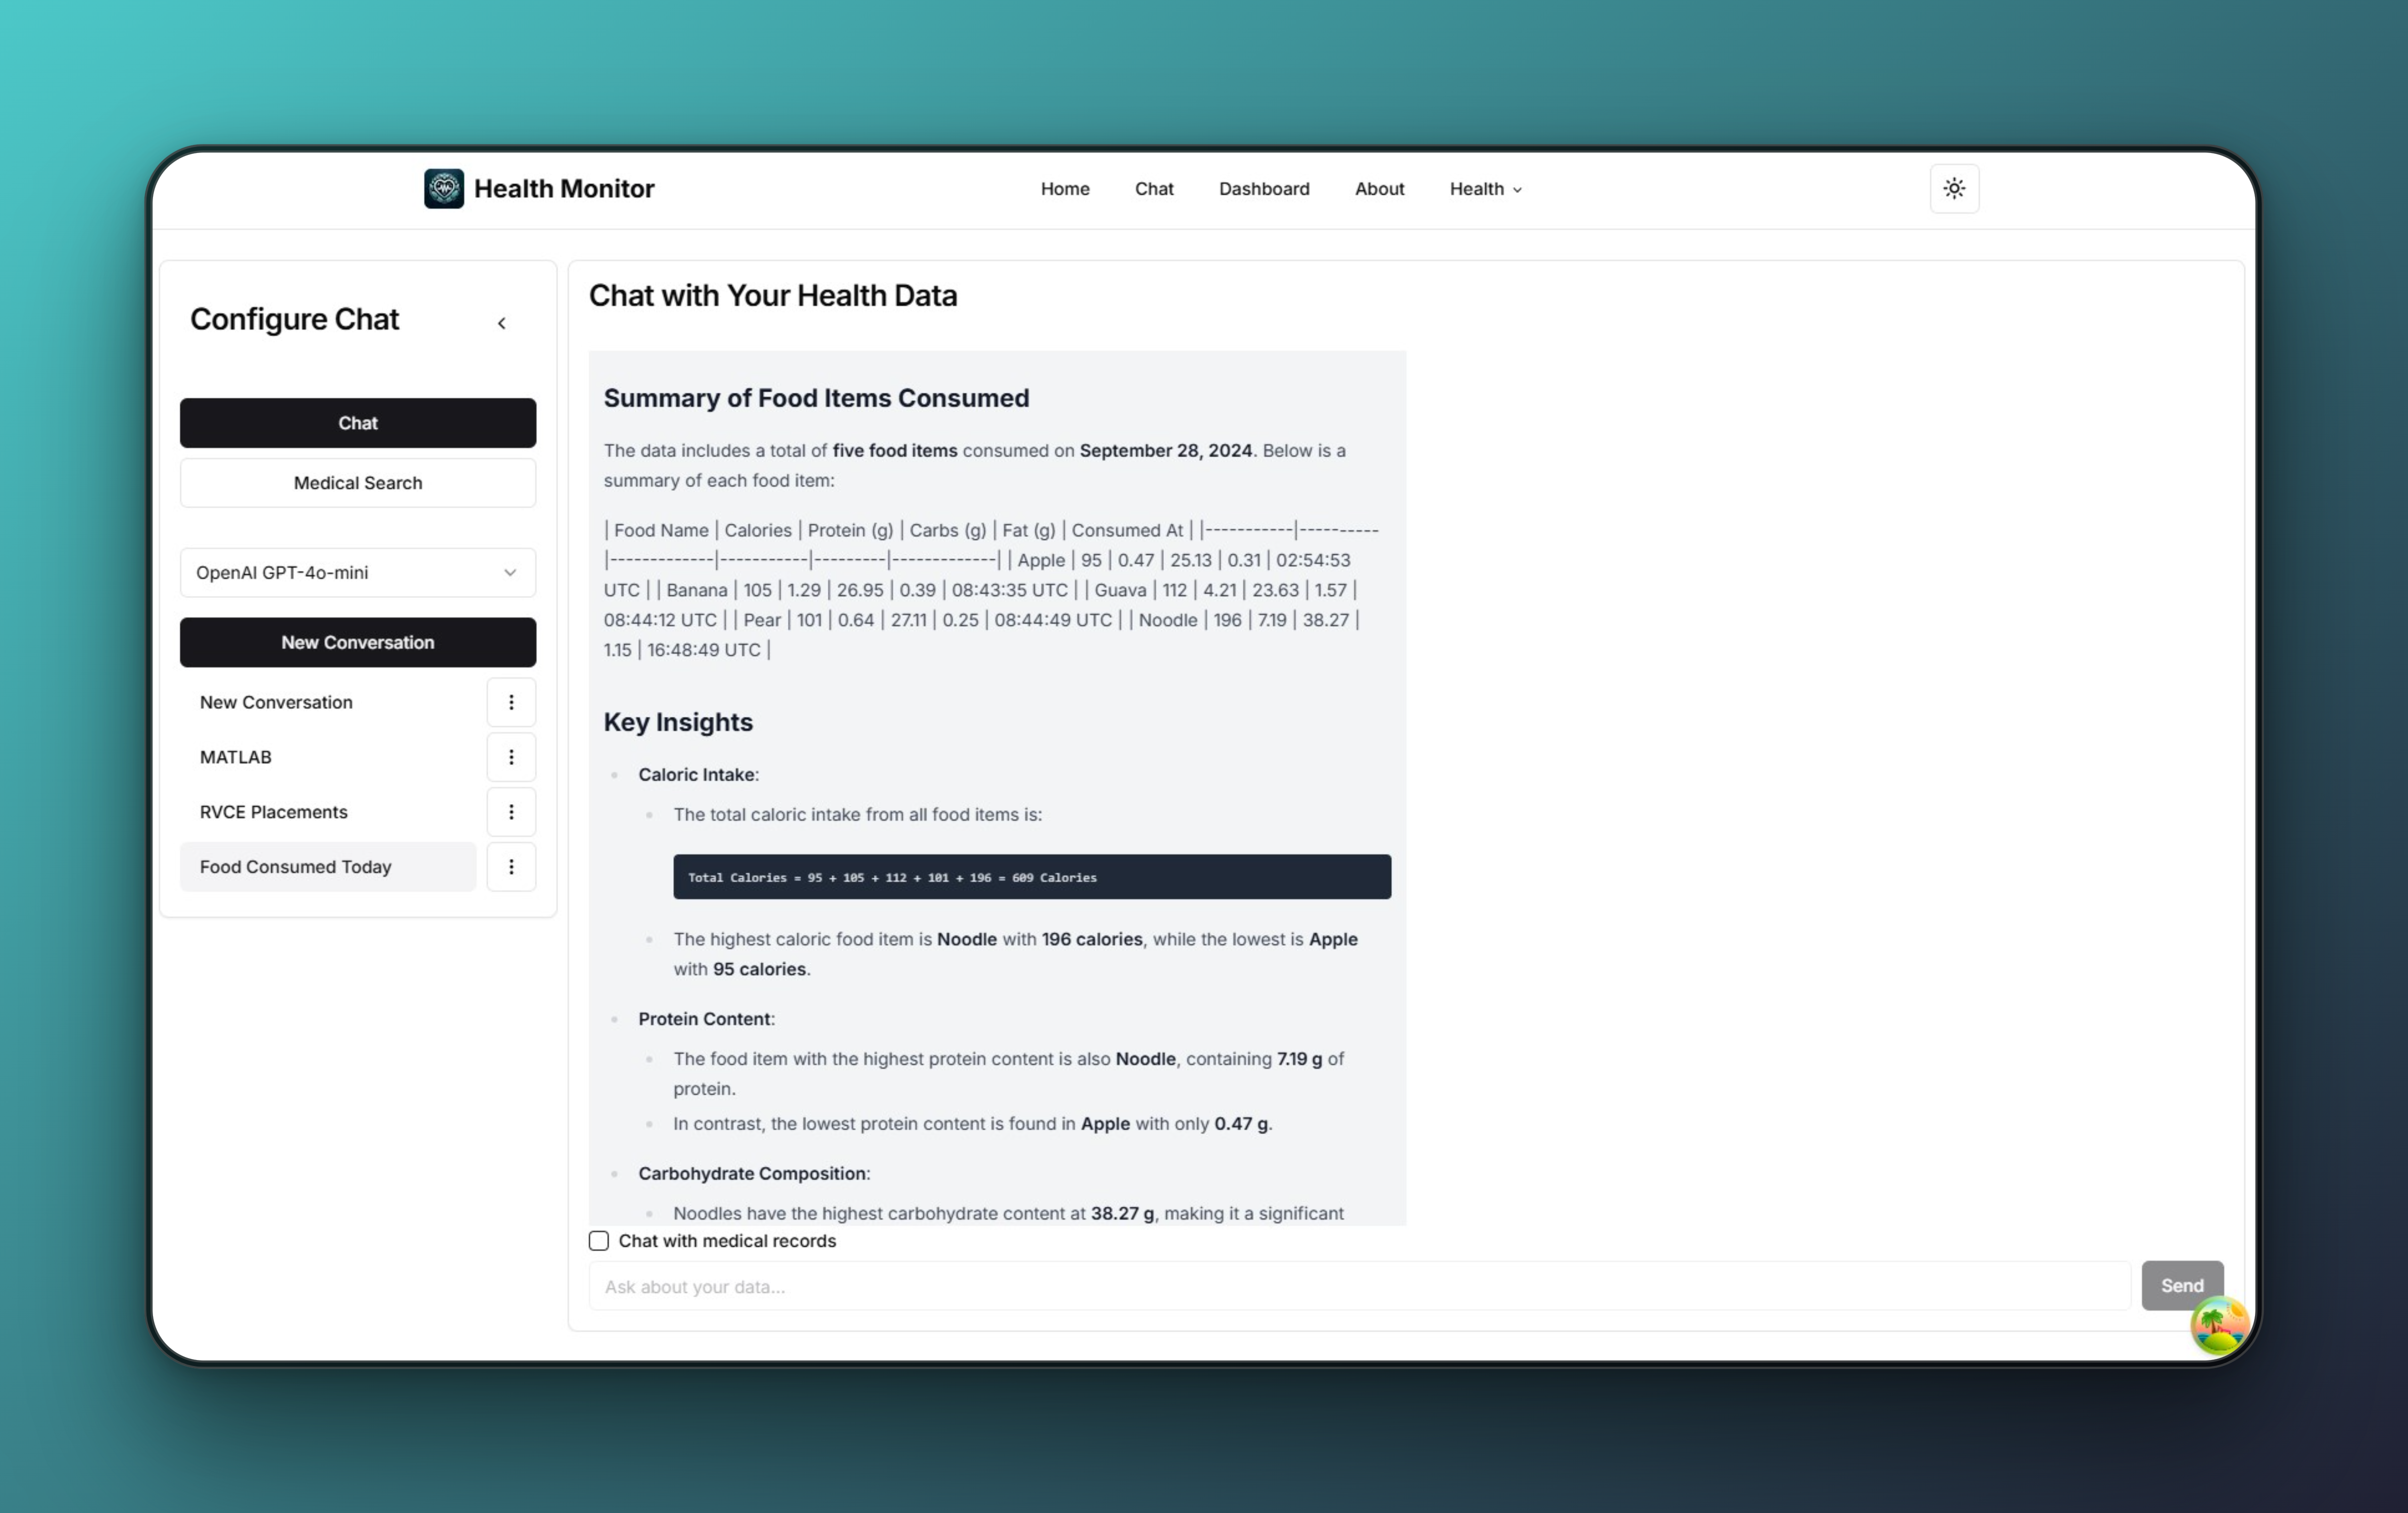
\includegraphics[width=\columnwidth]{figures/hm-chat-light}
\caption{AI-Powered Chat Interface with RAG Integration}
\label{fig:chat-interface}
\end{figure}

\begin{figure}[!t]
\centering
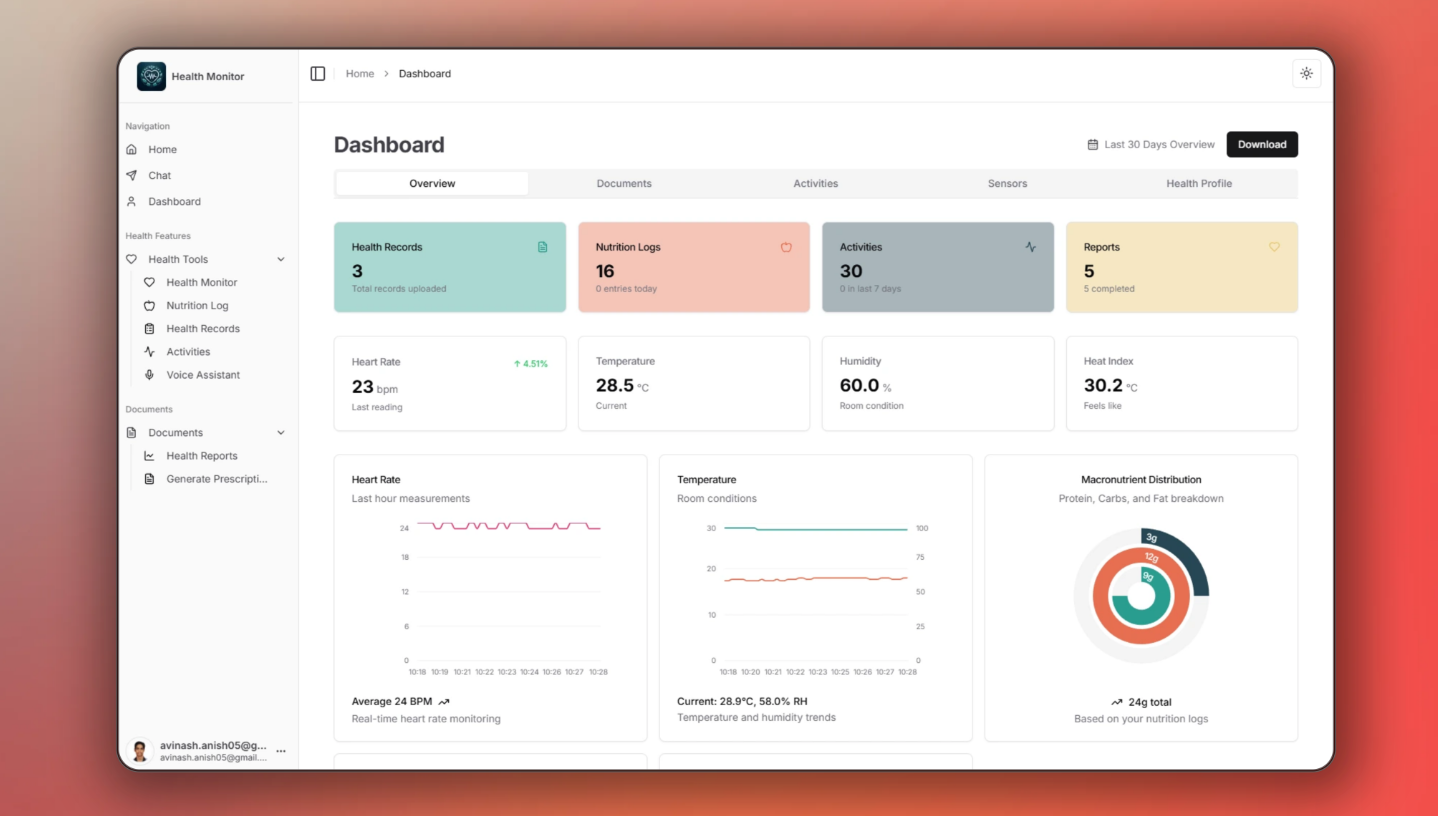
\includegraphics[width=\columnwidth]{figures/hm-dashboard}
\caption{Health Data Dashboard with SQL Agent Integration}
\label{fig:dashboard}
\end{figure}

The implementation demonstrates the successful integration of RAG pipeline and SQL agent technologies in a practical healthcare application, providing an intuitive interface for accessing and analyzing both structured and unstructured health data. 